\documentclass[twoside]{article}
\setlength{\oddsidemargin}{0.25 in}
\setlength{\evensidemargin}{-0.25 in}
\setlength{\topmargin}{-0.6 in}
\setlength{\textwidth}{6.5 in}
\setlength{\textheight}{8.5 in}
\setlength{\headsep}{0.75 in}
\setlength{\parindent}{0 in}
\setlength{\parskip}{0.1 in}

\usepackage{graphicx}
\usepackage{url}
\usepackage{amsmath}

%
% The following commands sets up the lecnum (lecture number)
% counter and make various numbering schemes work relative
% to the lecture number.
%
\newcounter{lecnum}
\renewcommand{\thepage}{\thelecnum-\arabic{page}}
\renewcommand{\thesection}{\thelecnum.\arabic{section}}
\renewcommand{\theequation}{\thelecnum.\arabic{equation}}
\renewcommand{\thefigure}{\thelecnum.\arabic{figure}}
\renewcommand{\thetable}{\thelecnum.\arabic{table}}
\newcommand{\dnl}{\mbox{}\par}

%
% The following macro is used to generate the header.
%
\newcommand{\lecture}[4]{
  \pagestyle{myheadings}
  \thispagestyle{plain}
  \newpage
  \setcounter{lecnum}{#1}
  \setcounter{page}{1}
  \noindent
  \begin{center}
  \framebox{
     \vbox{\vspace{2mm}
   \hbox to 6.28in { {\bf COMPSCI~590S~~~Systems for Data Science
                       \hfill Fall 2017} }
      \vspace{4mm}
      \hbox to 6.28in { {\Large \hfill Lecture #1: #2  \hfill} }
      \vspace{2mm}
      \hbox to 6.28in { {\it Lecturer: #3 \hfill Scribe(s): #4} }
     \vspace{2mm}}
  }
  \end{center}
  \markboth{Lecture {#1}: #2}{Lecture {#1}: #2}
  \vspace*{4mm}
}

%
% Convention for citations is authors' initials followed by the year.
% For example, to cite a paper by Leighton and Maggs you would type
% \cite{LM89}, and to cite a paper by Strassen you would type \cite{S69}.
% (To avoid bibliography problems, for now we redefine the \cite command.)
%
\renewcommand{\cite}[1]{[#1]}

% \input{epsf}

%Use this command for a figure; it puts a figure in wherever you want it.
%usage: \fig{NUMBER}{FIGURE-SIZE}{CAPTION}{FILENAME}
\newcommand{\fig}[4]{
           \vspace{0.2 in}
           \setlength{\epsfxsize}{#2}
           \centerline{\epsfbox{#4}}
           \begin{center}
           Figure \thelecnum.#1:~#3
           \end{center}
   }

% Use these for theorems, lemmas, proofs, etc.
\newtheorem{theorem}{Theorem}[lecnum]
\newtheorem{lemma}[theorem]{Lemma}
\newtheorem{proposition}[theorem]{Proposition}
\newtheorem{claim}[theorem]{Claim}
\newtheorem{corollary}[theorem]{Corollary}
\newtheorem{definition}[theorem]{Definition}
\newenvironment{proof}{{\bf Proof:}}{\hfill\rule{2mm}{2mm}}

% Some useful equation alignment commands, borrowed from TeX
\makeatletter
\def\eqalign#1{\,\vcenter{\openup\jot\m@th
 \ialign{\strut\hfil$\displaystyle{##}$&$\displaystyle{{}##}$\hfil
     \crcr#1\crcr}}\,}
\def\eqalignno#1{\displ@y \tabskip\@centering
 \halign to\displaywidth{\hfil$\displaystyle{##}$\tabskip\z@skip
   &$\displaystyle{{}##}$\hfil\tabskip\@centering
   &\llap{$##$}\tabskip\z@skip\crcr
   #1\crcr}}
\def\leqalignno#1{\displ@y \tabskip\@centering
 \halign to\displaywidth{\hfil$\displaystyle{##}$\tabskip\z@skip
   &$\displaystyle{{}##}$\hfil\tabskip\@centering
   &\kern-\displaywidth\rlap{$##$}\tabskip\displaywidth\crcr
   #1\crcr}}
\makeatother

% **** IF YOU WANT TO DEFINE ADDITIONAL MACROS FOR YOURSELF, PUT THEM HERE:



% Some general latex examples and examples making use of the
% macros follow.

\begin{document}

%FILL IN THE RIGHT INFO.
%\lecture{**LECTURE-NUMBER**}{**DATE**}{**LECTURER**}{**SCRIBE**}
\lecture{18}{SparkSQL}{Emery Berger}{Shamanth Kumar, Yichi Zhang}

In this lecture, we first discussed about SparkSQL which is a new module in Apache Spark that integrates relational processing with Spark’s functional programming API and its advantages. Then we talked about some basic concepts of complier.

\section{Disadvantages of using HiveQL}

1) Hive creates UDF(User Defined Functions) and UDAF(User Defined Aggregation Functions) as Java. This operation is a big ask for Java as Java is mostly static.\newline
2) UDF is a black box and it cannot be optimized.
3) HiveQL creates a bridge between SQL and MapReduce. It doesnot integrate them.\newline
4) It has more disk I/O.

%Some of other requirements of multiple processing which are hard to implement include:
%\begin{itemize}
   % \item Discovery mechanism (at the start)
    %\item Dynamic partitioning of heap
    %\item Load balancing
    %\item Fault-tolerance (synchronous checkpoints)
%\end{itemize}


\section{SparkSQL}

Spark SQL is similar to Hive, in that it provides a SQL interface on top of a MapReduce system. However,
while Hive’s API focuses only on providing SQL functionality, Spark SQL provides other functionality in
addition to SQL.

\section{Spark}

Spark is a cluster computing framework for Scala that provides MapReduce functionality and distributed data storage. High performance and fault tolerance are provided using RDDs (resilient distributed datasets), which are kept in memory (to the extent possible) during computation.  The main advantage of using Spark as compared to Hive is that it reduces the amount of I/O and hence is faster compared to Hive.\newline

Instead of replacing Spark code with a SQL API (the way Hive replaces Hadoop code with SQL),  Spark allows users to intermix SQL-like operations with Spark code. All parts of the resulting plan (both Spark and SQL code) are optimized. Spark SQL provides the DataFrame API, which basically corresponds to a SQL table. These DataFrames can be created from Spark RDDs or from external sources, and can be passed to and from Spark code/libraries.

Spark is written in a programming language called Scala. Scala runs on JVM(Java Virtual Machine). Examples of other JVM languages are Clojur and Kotlin. Scala is more advanced as compared to Java. Scala builds DSL's(Domain Specific Language).



\subsection{Macros in Scala}

Macros in Scala are turned into Abstract Syntax Trees(AST) which can generate code. There are no macros in Java.

\section{Complier}

We discussed basic concepts of complier. Compiler is used to transform source code (usually high level programming language e.g. Java, C) to target code (e.g. assembly language).

\begin{figure}[h]
\centering
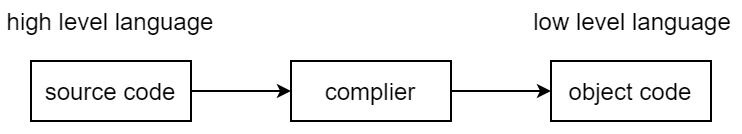
\includegraphics[scale=0.35]{compiler.png}
\caption{Compiler}
\end{figure}

Compiling has four basic stages: lexical analysis, parsing, complier logic, code generation. 

\begin{enumerate}

\item Lexical analysis :
Compiler scans the source code and converts characters to meaningful tokens. Common tokens include reserved word in certain language, such as "new", "if", "while" etc. in Java. For example, it takes 'w', 'h', 'i', 'l', 'e' into integer 15 which represents keyword "while".

\item Parsing : 
Also called syntax analysis, converts sequences of tokens into formal grammar, abstract syntax tree (AST). A statement can be parsed as followings:
\begin{equation*}
\begin{aligned}
\text{statement} &::= \text{varname assign expr} \\
\text{expr} &::= \text{number} | \text{expr binary\_op expr} | \text{unary\_op expr} | \text{expr} | \text{varname}
\end{aligned}
\end{equation*}
For example, given a statement $x = 9 + (y * 6)$:

\begin{figure}[h]
\centering
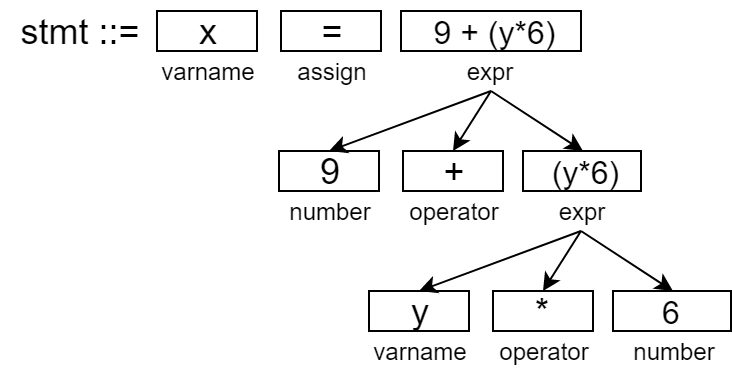
\includegraphics[scale=0.35]{AST.png}
\caption{Example of an AST}
\end{figure}

\item Complier logic and code generation:
Compiler then optimizes AST, generates intermediate representation(IR) and finally genrerates assembly code. Several optimization methods:
\begin{enumerate}
\item Constant folding in tree. For example, const operator const $\to$ const.
\item Inlining. Make small function inlined.
\item Dead code elimination.
\item Liveness analysis.
\item Strength reduction. Replacing expensive operations by cheaper operations. For example, replacing division 2 with right shift.
\end{enumerate} 

\begin{figure}[h]
\centering
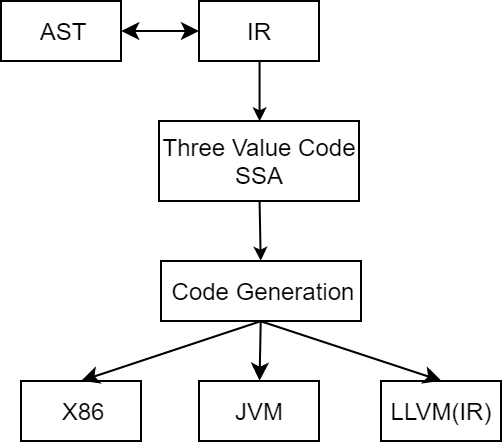
\includegraphics[scale=0.35]{code_generation.png}
\caption{CPU frequency scaling over the years}
\end{figure}

\end{enumerate}


\subsection{Strength Reduction}

Replacing expensive operations by cheaper operations.
Example: Division is an expensive operation.
              So, compiler replaces division operation in say, "/2" with right shift operator which is similar to division but cheaper compared to it.

\section{SparkSQL Optimizations}

Optimizer in SparkSQL is called a catalyst. Spark SQL operations on DataFrames are represented as abstract syntax trees (ASTs) of operations. Operations can be expressed with Scala quasiquotes, which Scala automatically parses into ASTs. Consider your program, pick an optimization, it gives you new AST, keep continuing the optimization process and stop it when converges i.e., when the AST's are equivalent. A real compiler does not do this but Spark SQL does.
Spark SQL optimizes SQL queries and optimizes UDF's using limited expression language as optimizing UDF's with Java is a high level job. All the SQL queries and all the expressions are compiled to a giant AST.

Several optimization techniques:

\begin{enumerate}

\item Predicate Pushdown

This query optimization takes predicate statements (e.g. "WHERE" clauses) and pushes them closer to the data source, so that less irrelevant data is retrieved as part of the SQL query.

\item Column Pruning

This query optimization moves the attributes selected closer to the data source, again to avoid retrieving unecessary data that won't actually be used.

\item Quasiquotes

Quasiquotes are a neat notation that lets you manipulate Scala syntax trees with ease:
scala> val tree = q"i am a quasiquote "
tree: universe.Tree = i.am(a.quasiquote)
Every time you wrap a snippet of code into q"..." quotation it would become a tree that represents given
snippet.


\end{enumerate}





%\begin{itemize}
   % \item Synchrony - This can be avoided by having many threads and thus we can hide latency by switching to other threads.
    %\item Concurrency - Locks provide exclusive access to a shared memory but the lock itself is in shared memory. This forms a kind of recursive problem and can be avoided by using a separate locking service.
%\end{itemize}


\end{document}